\section{Theoretische Grundlage}
\label{sec:Theorie}
Unter dem Zeemaneffekt wird die Aufspaltung der Energieniveaus der einzelnen Zustände, sowie die Polarisation des Lichtes verstanden. Dabei wird zwischen dem normalen und dem anomalen Zeemaneffekt differenziert. Im folgenden wird die theoretische Grundlage des Versuches skizziert.

\subsection{Magnetisches Moment eines Elektrons}
Elektronen besitzen sowohl einen Bahndrehimpuls $l$ sowie ein Eigendrehimpuls $s$. In der weiteren Betrachtung werden nur die Drehimpulse der äußeren Schalen der Atome betrachtet, da die der abgeschlossenen Schalen verschwinden. Ausgehend von der Eigenwertgleichung der Zustände des Atoms werden die Beträge der Quantenzahlen zu
\begin{eqnarray}
  |\vec{l}| = \sqrt{l(l+1)} \hbar  \\
  |\vec{s}| = \sqrt{s(s+1)} \hbar
  \label{eqn:betQua}
\end{eqnarray}
berechnet. Dabei laufen der Bahndrehimpuls $l$ von 0, 1, \ldots $\,$ n-1 und der Spin $s$ ist $\frac{1}{2}$. Für die Berechnung der Magnetischen Momenten wird das Borsche Magneton $\mu_\text{B}$ eingeführt welches eine Art infinitesimales magnetisches Moment ist. Es entspricht dem magnetischen Moment welche ein Elektron mit $l$=1 erzeugt. Das in Maßeinheiten des Magnetons berechnete magnetische Momente des Bahndrehimpuls beträgt
\begin{equation}
  \vec{\mu_\text{L}} = -\mu_\text{B} \sqrt{l(l+1)} \vec{l_\text{e}} \ .
  \label{eqn:magL}
\end{equation}
Bei der Einführung des magnetischen Moment des Spins $\mu_\text{s}$
\begin{equation}
  \mu_\text{s} = - \mu_\text{B} g_\text{S} \sqrt{s(s+1)} \vec{s_\text{e}}
  \label{eqn:magS}
\end{equation}
tritt der Landé-Faktor $g_\text{S}$ auf, auf welchen im folgenden noch weiter eingegangen wird.

\subsection{Wechselwirkungen der Drehimpulse untereinander}
Bei den Wechselwirkungen der einzelnen Drehimpulse untereinander wird unterschieden zwischen zwei verschiedenen Fällen die fließend ineinander übergehen.  Bei dem ersten Fall wird davon ausgegangen, dass die Kernladungszahl so niedrig ist. Die Wechselwirkungen zwischen den einzelnen $\vec{l_\text{i}}$ st so gering, dass ein Gesamtdrehimpuls $\vec{L}$ eingeführt werden kann.
\begin{equation}
  \vec{L} = \sum \vec{l_\text{i}}
  \label{eqn:L}
\end{equation}
Dabei sind jegliche vektoriellen Additionen der einzelnen Bahndrehimpulse $l_\text{i}$ erlaubt bei denen der Gesamtdrehimpuls eine ganzzahlige Zahl ist. In analogie zu den einzelnen Drehimpulsen wird das magnetische Moment
\begin{equation}
  |\mu_\text{L}| = \mu_\text{B} \sqrt{L(L+1)}
  \label{magL}
\end{equation}
des Gesmatbahndrehimpuls eingeführt. Analog zum Bahndrehimpuls wird auch eine Gesamtspinquantenzahl $S$ als auch ein magnetisches Moment $\mu_\text{S}$ eingeführt . Für nicht zu großen Magnetfelder lässt sich der Gesamtdrehimpuls $\vec{J}$ aus der Summe von $L$ und $S$ einführen welcher auch als LS-Kopplung bezeichnet wird.
Der zweite Fall der Kopplung von Spin und Bahndrehimpuls wird als j-j-Kopplung bezeichnet. Dabei wird angenommen das bei schweren Atomen die Wechselwirkung des Spins und des Bahndrehimpuls untereinander so groß wird, dass diese nicht mehr vernachlässigt werden kann. Somit müssen die einzelnen Gesamtdrehimpuls
\begin{equation}
  \vec{j_\text{i}} = \vec{l_\text{i}} + \vec{s_\text{i}}
  \label{eqn:j}
\end{equation}
berücksichtigt werden, sodass der Gesamtdrehimpuls $\vec{J}$ die Summe der einzelnen $\vec{j_\text{i}}$ ist.

\subsection{Aufspaltung der Energieniveaus}
Das magnetisches Moment des Gesamtdrehimpuls ist die Summe des Spins $\mu_\text{s}$ und des magn. Momets $\mu_\text{l}$.
\begin{equation}
  \mu = \mu_\text{l} + \mu_\text{l}
\end{equation}
Da der Landé-Faktor bei Elektronen welche ein Spin 1/2 haben meist den Wert 2 besitzt, zeigen $\mu$ und $J$ im Regelfall nicht in die gleiche Richtung. Jedoch oszilliert das magnetische Moment um die Achse von $J$ sodass im Zeitmittel die Richtung von $\vec{\mu}$ nicht von $\vec{J}$ zu unterscheiden ist. Für den Betrag von $\mu_\text{J}$ ergibt sich
\begin{equation}
  |\vec{\mu_\text{J}}| = \mu_\text{B} g_\text{J} \sqrt{J(J+1)} \ ,
  \label{eqn:muJ}
\end{equation}
wobei $g_\text{J}$ der Landé-Faktor ist. Dieser ist definiert als
\begin{equation}
  g_\text{J} = \frac{3J(J+1) + S(S+1) -L(L+1)}{2J(J+1)}
  \label{eqn:Lan}
\end{equation}
Die Richtungsquantelung besagt das nur solche Winkel auftreten können bei dennen der Winkel zwichen $\vec{\mu}$ und $\vec{B}$ ein ganzzahliges Vielfaches von
\begin{equation}
\vec{\mu} = -m g_\text{J} \mu_\text{B},
  \label{eqn:mu}
\end{equation}
ist, wobei  $m  = (-J, \cdots, J)$ läuft. Somit Spaltet sich die Energieniveaus im Magnetfeld in $2J+1$ Niveaus auf, deren Energiedifferenzen zum Magnetfreien Niveau
\begin{equation}
	\Delta E_\text{mag} = m \vec{\mu_\text{B}} \vec{g_\text{J}}
  \label{eqn:delE}
\end{equation}
Ein Beispiel für die Aufspaltung eine Niveaus mit $J=2$ ist in Abbildung \ref{fig:Eniv} zu sehen.
\begin{figure}
  \centering
  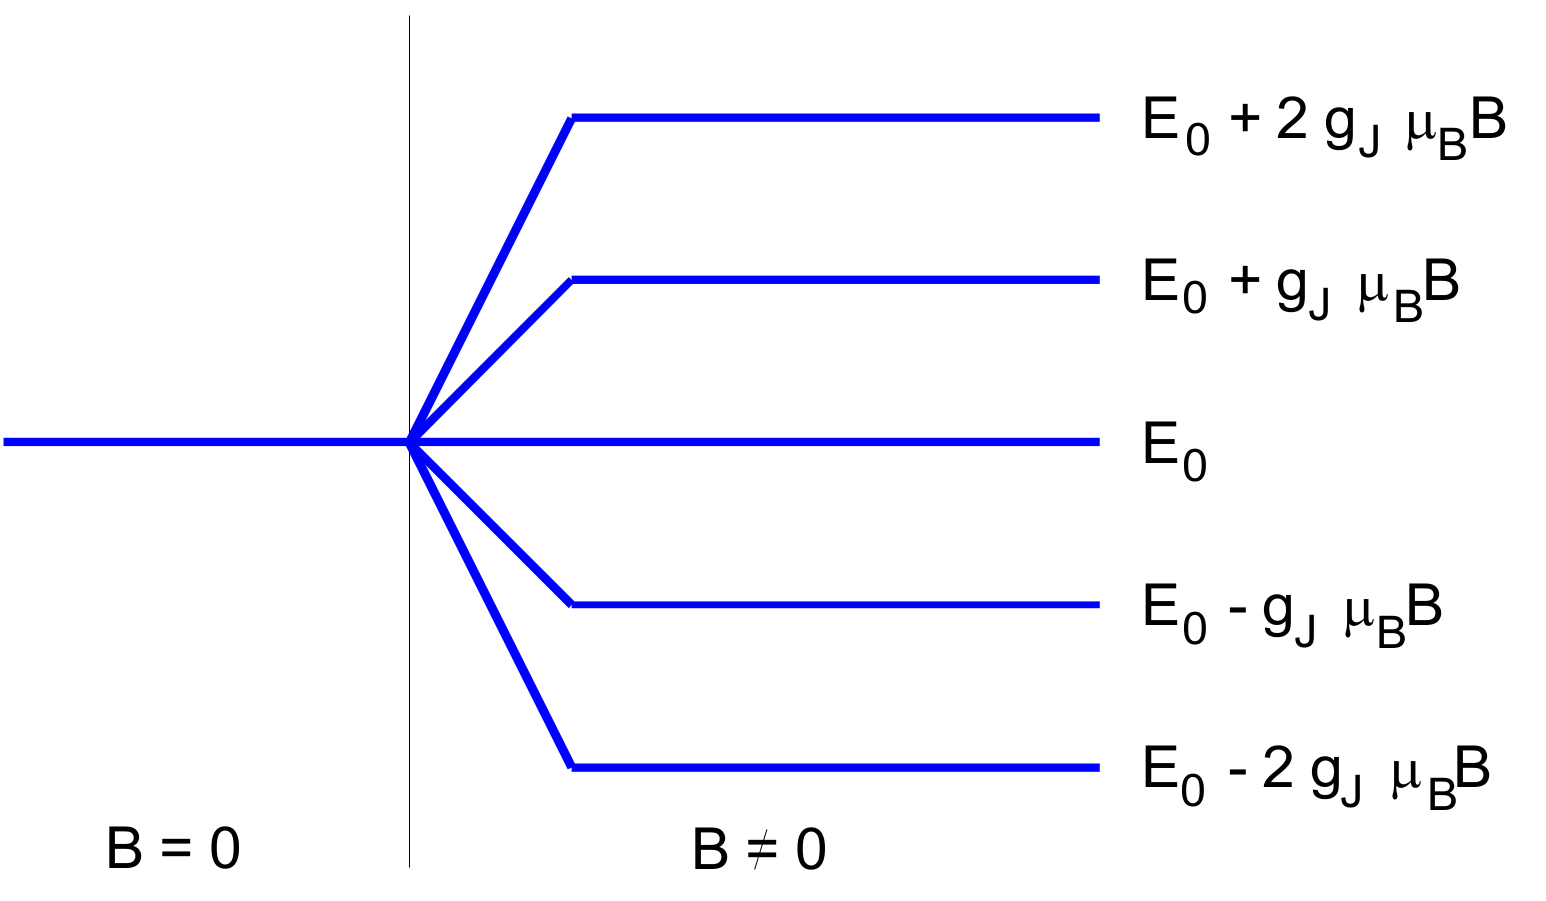
\includegraphics[height=6cm]{./Bilder/ENiveaus.png}
  \caption{Aufspaltung der Energieniveaus im Magnetfeld \cite{V27}}
   \label{fig:Eniv}
\end{figure}

\subsection{Auswahlregeln}
Mithilfe der Schrödingergleichung wird untersucht welche Niveauübergänge möglich sind. Als Ansatz zur Lösung wird die Summe zweier Ebenen Wellen genommen bei denen der Spin berücksichtigt wird. Aus der Dichtefunktion lässt sich ablesen, dass die Elektronen mit der Frequenz $\nu_{\alpha\beta}$ zwischen den beiden Energiezuständen oszillieren.
\begin{equation}
  \nu_{\alpha\beta}= \frac{E_{\alpha} - E_{\beta}}{\hbar}
  \label{eqn:nu}
\end{equation}
Zur Berechnung des Dipolmoment die das Elektron durch die Schwingung zwischen den E-Niveaus ausführt wird, muss die Gleichung
\begin{equation}
  -e_0\, x \, \Psi^* \Psi \, \text{dV}
  \label{}
\end{equation}
gelöst werden. Anhand der Lösung kann aus dem Poyntingvektor abgeleitet werden das alle Beiträge verschwinden, außer wenn m die Zahlenwerte
\begin{equation}
  \Delta m = -1,0,1
\end{equation}
annimmt. Aus der Herleitung lässt sich schließen das für $m = \pm 1$ das Licht zirkular ist. Dieser Übergang wird $\sigma^{+/-}$ genannt, entsprechemd des vorzeichens von $m$. Aufgrund der zikularen Polarisation ist das Feld sowohl longitudinal als auch Transversal zu beobachten. Bei $\pi$ Übergang ist $m = 0$ wobei nur eine Transversale Schwingung zu beobachten ist. Somit können die beiden Felder in der Versuchsdurchführung differenziert werden.

\subsection{Normaler Zeeman-Effekt}
Beim normalen Zeeman-Effekt verschwindet die Summe der einzelnen Spins ($S=0$), sodass der entsprechende Landé-Faktor für alle $J : g_\text{J} = 1$ ist. Dabei ist die Aufspaltung der einzelnenEnergieniveaus unabhängig von der Quantenzahl. Die Energiedifferenz der Übergänge kann mittels Formel \ref{eqn:delE} berechnet werden.
\subsection{Anomale Zeeman-Effekt}
Ist der Atomspin von Eins verschieden, wird vom Anomalen Zeeman-Effekt gesprochen. Bei diesem kommt es aufgrund der Landé-Faktoren welcher von null verschieden ist zu mehr Aufspaltungen als beim normalen Zeeman-Effekt. Die Energiedifferenz der einzelenen Niveaus lässt sich durch die Formel
\begin{equation}
  \Delta E = \mu_\text{B}\,B\,(m_1 g_1 + m_2 g_1)
  \label{eqn:dE}
\end{equation}
berechenen.

\subsection{Fehlerrechnung}
Sämtliche Fehlerrechnungen werden mit Hilfe von Python 3.4.3 durchgeführt.
\subsubsection{Mittelwert}
Der Mittelwert einer Messreihe $x_\text{1}, ... ,x_\text{n}$ lässt sich durch die Formel
\begin{equation}
	\overline{x} = \frac{1}{N} \sum_{\text{k}=1}^\text{N} x_k
	\label{eqn:ave}
\end{equation}
berechnen. Die Standardabweichung des Mittelwertes beträgt
\begin{equation}
	\Delta \overline{x} = \sqrt{ \frac{1}{N(N-1)} \sum_{\text{k}=1}^\text{N} (x_\text{k} - \overline{x})^2}
	\label{eqn:std}
\end{equation}

\subsubsection{Gauß'sche Fehlerfortpflanzung}
Wenn $x_\text{1}, ..., x_\text{n}$ fehlerbehaftete Messgrößen im weiteren Verlauf benutzt werden, wird der neue Fehler $\Delta f$ mit Hilfe der Gaußschen Fehlerfortpflanzung angegeben.
\begin{equation}
	\Delta f = \sqrt{\sum_{\text{k}=1}^\text{N} \left( \frac{ \partial f}{\partial x_\text{k}} \right) ^2 \cdot (\Delta x_\text{k})^2}
	\label{eqn:var}
\end{equation}

\subsubsection{Lineare Regression}
Die Steigung und y-Achsenabschnitt einer Ausgleichsgeraden werden gegebenfalls mittels Linearen Regression berechnet.
\begin{equation}
	y = m \cdot x + b
	\label{eqn:reg}
\end{equation}
\begin{equation}
	m = \frac{ \overline{xy} - \overline{x} \overline{y} } {\overline{x^2} - \overline{x}^2}
	\label{eqn:reg_m}
\end{equation}
\begin{equation}
	b = \frac{ \overline{x^2}\overline{y} - \overline{x} \, \overline{xy}} { \overline{x^2} - \overline{x}^2}
	\label{eqn:reg_b}
\end{equation}
